\begin{figure}
    \centering
    \subfigure[1. Wirbelsatz \label{Wirbelringe:fig:Helmholtz_1}]{
        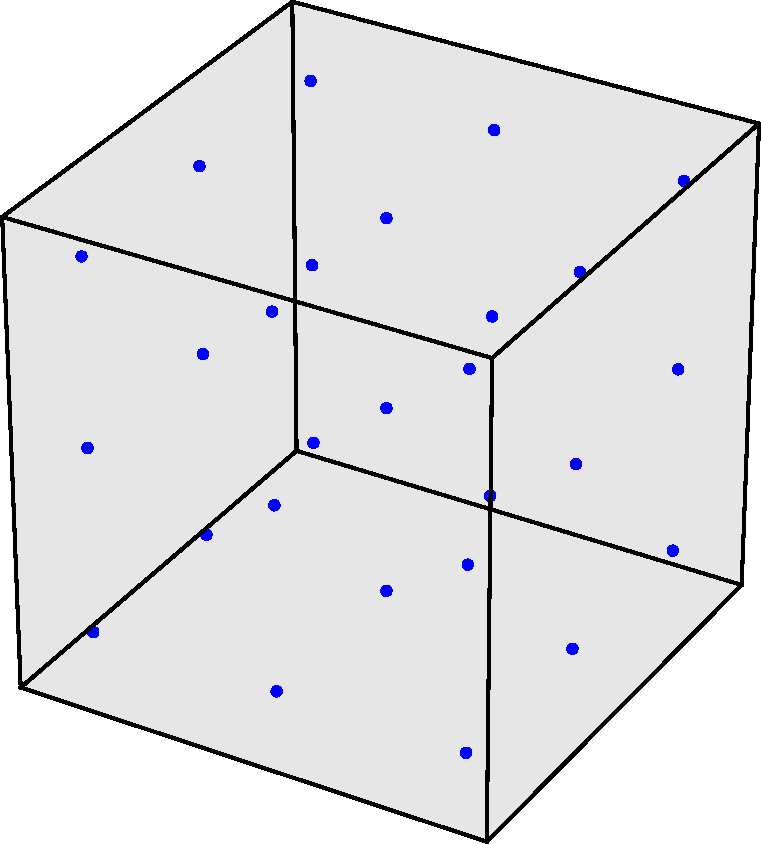
\includegraphics[width=0.3\textwidth]{papers/wirbelringe/fig/cube_still_particles.pdf}
    }\hfill
    \subfigure[2. Wirbelsatz \label{Wirbelringe:fig:Helmholtz_2}]{
        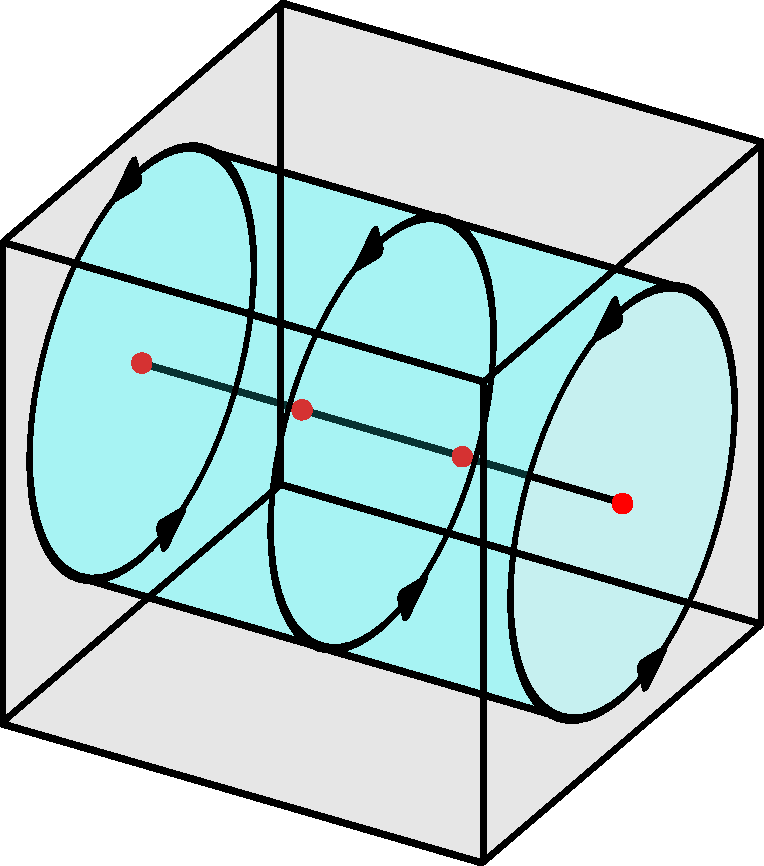
\includegraphics[width=0.3\textwidth]{papers/wirbelringe/fig/cube_still_particles_rotation.pdf}
    }\hfill
    \subfigure[3. Wirbelsatz \label{Wirbelringe:fig:Helmholtz_3}]{
        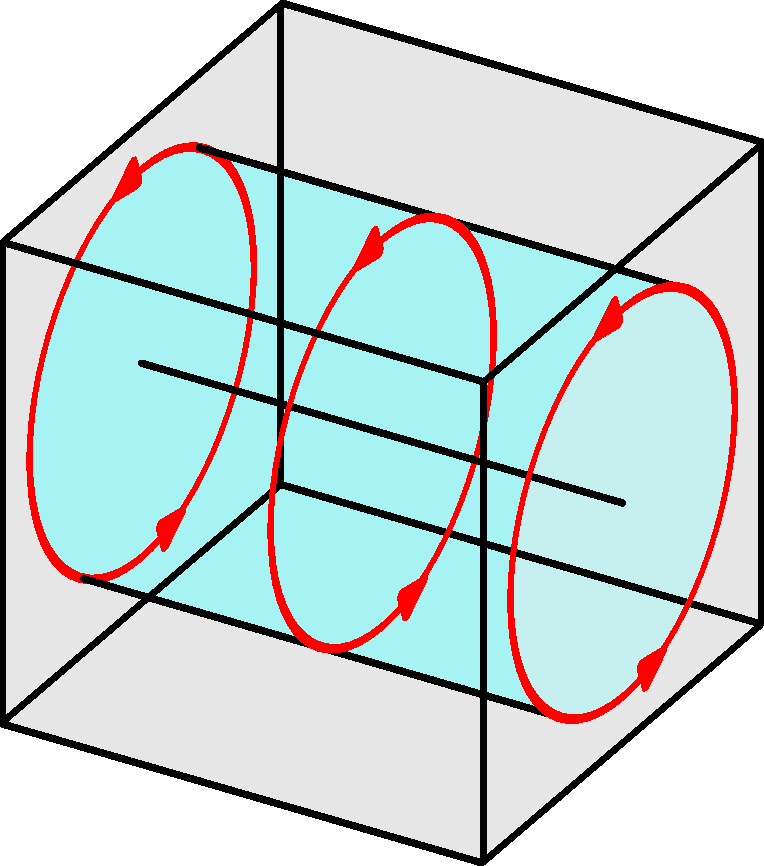
\includegraphics[width=0.3\textwidth]{papers/wirbelringe/fig/cube_constant_rotation.pdf}
    }
    \caption{Helmholtzsche Wirbelsätze visuell dargestellt in einem abgeschlossenen System mit idealen Grenzflächen.}
    \label{Wirbelringe:fig:Wirbelsaetze}
\end{figure}